

\tikzset{every picture/.style={line width=0.75pt}} %set default line width to 0.75pt        

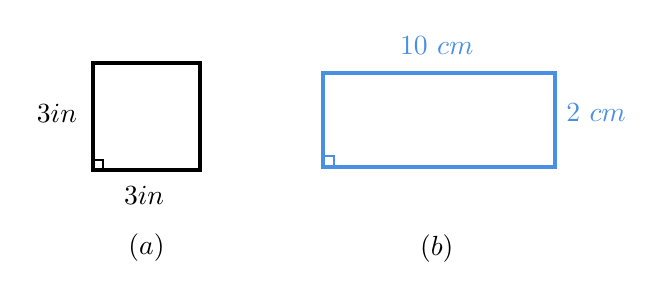
\begin{tikzpicture}[x=0.75pt,y=0.75pt,yscale=-1,xscale=1, scale=0.6]
%uncomment if require: \path (0,218); %set diagram left start at 0, and has height of 218

%Shape: Square [id:dp9958510811050907] 
\draw  [line width=1.5]  (135,45) -- (221,45) -- (221,131) -- (135,131) -- cycle ;
%Shape: Square [id:dp2209502611968972] 
\draw   (135,122.81) -- (143.19,122.81) -- (143.19,131) -- (135,131) -- cycle ;
%Shape: Rectangle [id:dp27912537729912623] 
\draw  [color={rgb, 255:red, 74; green, 144; blue, 226 }  ,draw opacity=1 ][line width=1.5]  (320,53) -- (506,53) -- (506,128) -- (320,128) -- cycle ;
%Shape: Square [id:dp059563169319218456] 
\draw  [color={rgb, 255:red, 74; green, 144; blue, 226 }  ,draw opacity=1 ] (320,119.81) -- (328.19,119.81) -- (328.19,128) -- (320,128) -- cycle ;

% Text Node
\draw (106,85) node   {$3\text{ in}$};
% Text Node
\draw (176,151) node   {$3\text{ in}$};
% Text Node
\draw (178,193) node   {$( a)$};
% Text Node
\draw (411,31) node   {$\textcolor[rgb]{0.29,0.56,0.89}{10\ \text{cm}}$};
% Text Node
\draw (539,85) node   {$\textcolor[rgb]{0.29,0.56,0.89}{2\ }\textcolor[rgb]{0.29,0.56,0.89}{\text{cm}}$};
% Text Node
\draw (411,194) node   {$( b)$};


\end{tikzpicture}